\documentclass{article}
\usepackage[margin=1.2in]{geometry}
\usepackage{graphicx}
\usepackage{placeins}
\usepackage{url}
\usepackage{hyperref}
\graphicspath{ {./images/} }

\begin{document}
\title{Graphing and Analyzing Little-Rock Temperatures, 2000 - 2022}
\author{Julia Hambuchen}
\date{April 4th, 2022}
\maketitle

\begin{abstract}
This report describes the process and results of analyzing around 20 years of weather data from Little Rock, Arkansas, USA. The data initally gathered gives the high, low, and average temperature of each day from January 1st, 2000 to January 1st, 2022. Sorting this data in Python, the record highs and lows are grabbed from these 22 years and the highs, lows, and averages are graphed respectively.
\end{abstract}

\section{Introduction}
The data pulled to complete this project comes from the NOAA (National Oceanic and Atmospheric Administration) online weather data, NOWData. It collects data recorded from stations all over the United States, including precipitation levels and snow depth \cite{NOWData}. However, only the daily highs, lows, and averages were used in this project. The main purpose of taking data from the beginning of the 2000's was to see if, in Little Rock, AR, 22 years would be a sufficent enough scope to see the effects of a warming climate. According to NASA, the National Aeronautics and Space Administration, weather and global climate can differ dramatically. While regional temperatures may fluctuate frequently, global temperature rises and regional temperatures follow along, albeit sometiems erraticly \cite{weather_vs_climate}. By analyzing these local highs, lows, and averages, we may or may not be able to notice a trend upwards. Regardless of seeing any trends, we will be able to make out the cyclic seasonal pattern through the 22 years, and see any noticeable highs / lows that occured. 


\section{Graphs for Yearly Record Temperatures}
For each year, we found the 'hottest' high and the 'coolest' low. These values were plotted side-by-side, with the y-axis showing temperature and the x-axis showing the years 2000 - 2021. 2022 was excluded in both the 'highest highs' and 'lowest lows' graphs, since the year's temperatures are not completed yet. The highest recorded temperatures are shown below. 2011 had the hottest year on record, reaching a temperature of 114 degrees Farenheit on August 3rd, 2011. This value was confirmed with an article from the Arkansas Democrat Gazette talking about the intense heat on August 4th, 2011 \cite{historic_high}.

\begin{figure}[h!]
\centering
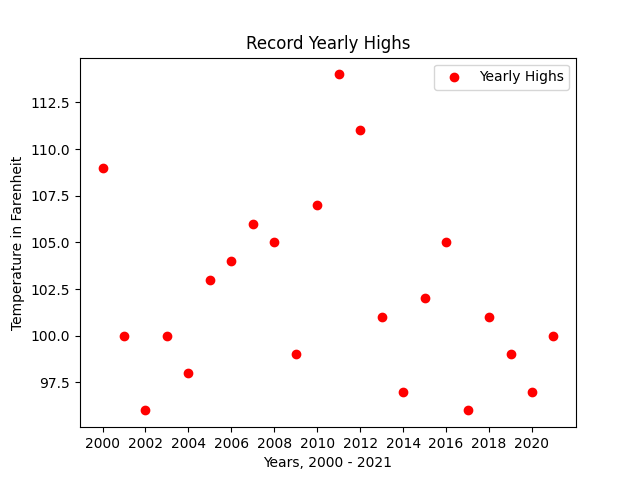
\includegraphics[scale=0.8]{Highs.png}
\label{Figure 1: Record Highs}
\caption{Figure 1: Record Highs, data from NOWData.}
\end{figure}
\FloatBarrier

\begin{figure}[h!]
\centering
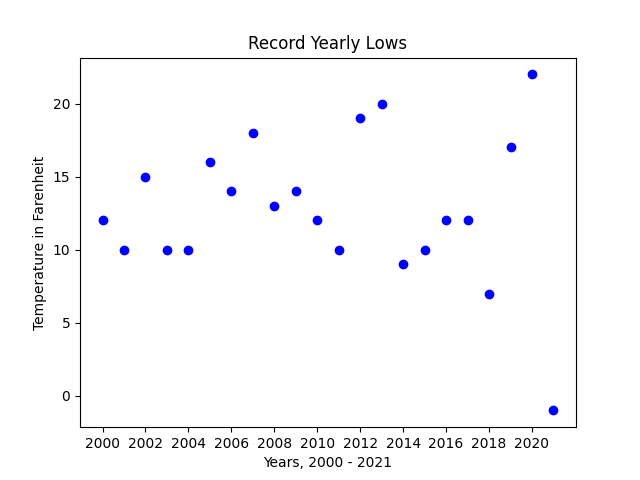
\includegraphics[scale=0.8]{Lows.png}
\label{Figure 2: Record Lows}
\caption{Figure 2: Record Lows, data from NOWData.}
\end{figure}
\FloatBarrier

Figure 2 shows the years' lowest lows, with the record being recently on Febuary 16th, 2021, at -1 degrees Farenheit.


\section{Graphs for Average Temperatures over Time}
Graphing all the daily averages over January 1st, 2000 - January 31st, 2022 results in a cyclic pattern that shows the transition from winter, to spring, to summer, to fall, to winter again over and over. Here it is below:

\begin{figure}[h!]
\centering
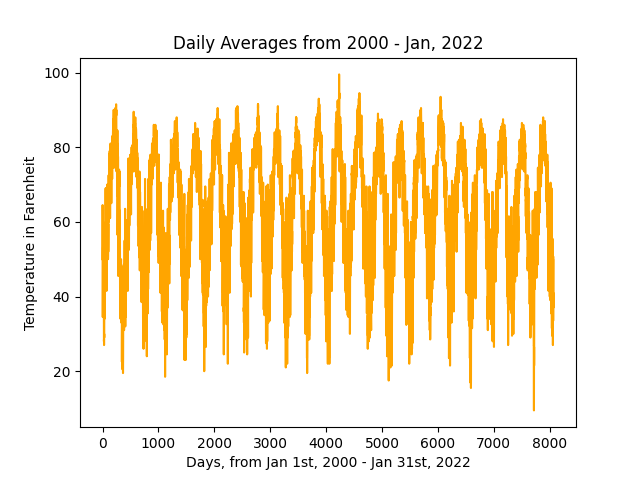
\includegraphics[scale=0.8]{Averages.png}
\label{Figure 3: Daily Averages}
\caption{Figure 3: Daily Averages, data from NOWData.}
\end{figure}
\FloatBarrier


\section{Conclusions}
Looking at our graphs for Little Rock highs, lows, and averages over 21-ish years, we can see no significant increase oor decrease in temperatures overall. There were very general trends for the record highs and lows over the years, but the overall data was too sporadic to give these trends much merit. Just like looking at a picture way too closely, by narrowing in on a two-decade range, it is hard to tell if we are getting the 'big picture.' Regional areas are more erratic than global temperature in that it goes through seasonal variations and is subject to variations like La Nina and El Nino years \cite{el_la_nino_nina}, natural cycles that produce cooler and warmer weather periodically. There are several factors that play into regional temperatures, but global temperature is much more stagnant and a better measure of changes in climate \cite{weather_vs_climate}.


\bibliographystyle{plain}
\bibliography{weather_bib}

\end{document}
